\section{Optimisation}
\subsection{Caching}
\subsubsection{Redis}
\begin{figure}[H]
    \begin{minipage}{.3\textwidth}
      
\includegraphics[width=1\linewidth]{img/redis.png}
    \end{minipage}
    \begin{minipage}{.7\textwidth}
Redis est une base de données NoSQL mais elle n'est pas très similaire aux autres bases de données NoSQL. Cela est dû au fait que Redis ne fonctionne pas vraiment avec des tables, mais toutes les données dans Redis sont stockées dans des paires clé-valeur. 
Il y a donc une clé ayant un nom et une valeur appelée Kyle.
L'objectif n'est donc pas de stocker un ensemble de données structurées, mais simplement de stocker une paire clé-valeur individuelle à partir de laquelle nous pouvons accéder aux données.
Il est important de noter que Redis fonctionne en utilisant la mémoire RAM de la machine sur laquelle il tourne, cela signifie qu'il est extrêmement rapide.
\newpara
Dans le cas où nous devons accéder à des informations qui prennent beaucoup de temps à charger, par exemple une quantité de données assez importante provenant de la base de données, nous pouvons utiliser Redis pour stocker ces valeurs pendant une durée définie. Ainsi, lorsque nous devrons accéder à cette même information, la réponse sera beaucoup plus rapide puisque l'information sera déjà chargée.
\end{minipage}
\end{figure}
\subsubsection{Analyse des résultats}
Le temps de chargement des données sur certaines de mes API était assez important et je devais trouver une solution pour le réduire. 
Afin d'améliorer le temps de chargement des données, j'ai décidé d'utiliser Redis. 
Pour tester Redis, j'ai décidé de récuperer tous les clients se trouvant dans ma base de données, ce qui correspond à, environ, 1400 clients.

\subsubsubsection{Sans utilisation de Redis}
Dans la figure ci-dessous, nous pouvons voir que le temps de réponse de la requête réalisée sans Redis a tendance à diminuer un peu après la première requête. Ceci est dû à la gestion du cache de Sequelize et de Postgres. Bien que ce temps ait diminué, la moyenne de ces temps est encore élevée, elle correspond à 495 ms, une demi-seconde.
\begin{figure}[H]
    \centering
    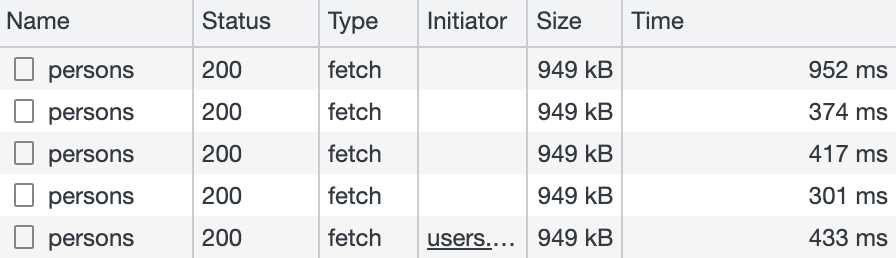
\includegraphics[width=\linewidth]{img/sans-redis.png}
    \caption{Temps de réponse sans Redis}
    \label{Sans-Redis}
  \end{figure}
\subsubsubsection{Avec utilisation de Redis}
La même requête a été faite mais cette fois avec Redis. Dans la figure 5, la première requête, sans Redis, dure une seconde, ce qui est assez conséquant. Les requêtes suivantes utilisant Redis diminuent considérablement en obtenant une moyenne de 204ms.
\begin{figure}[H]
    \centering
    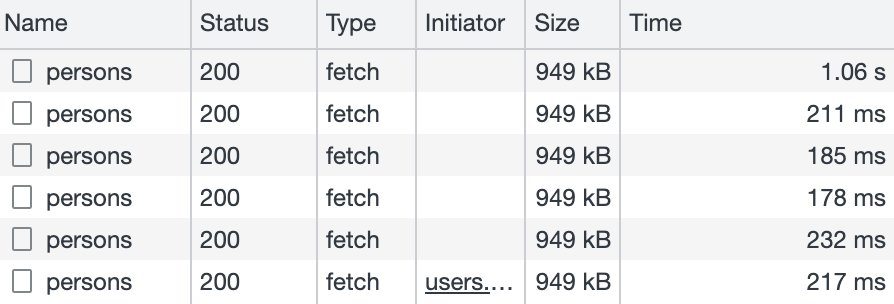
\includegraphics[width=\linewidth]{img/avec-redis.png}
    \caption{Temps de réponse avec Redis}
    \label{Avec-Redis}
\end{figure}
La performance obtenue en utilisant redis a augmenté d'un 58,8\%.

